\section{Topology Selection}
Starting the design, the topology selection must be covered first. The five isolated DC-DC converter topologies that were covered in the lectures are listed with their strengths and weaknesses in Table \ref{tab:procon}\cite{web:keysan}.
\renewcommand{\arraystretch}{1.5}
\begin{table}[H]

\centering
\caption{Comparison of Isolated DC-DC Converter Topologies}
\label{tab:procon}
\begin{tabular}{|m{0.2\textwidth}<{\centering}|m{0.35\textwidth}|m{0.35\textwidth}|}
    \hline
    \textbf{Topology} & \centering \textbf{Advantages} & \centering \textbf{Disadvantages} \arraybackslash \\ \hline
    
    \multirow{4}{*}{Flyback} & $\bullet$ Two-winding transformer & $\bullet$ High MOSFET voltage stress\\
    & $\bullet$ Low component count & $\bullet$ Low controllability \\ 
    & $\bullet$ Analog ICs are available for the duty cycle control & $\bullet$ Needs snubber due to leakage and parasitic inductances at primary side \\ \hline
    
    \multirow{3}{*}{Forward} & \multirow{3}{0.35\textwidth}{\justifying $\bullet$ $L_m$ has a discharge path on the auxiliary winding, no need for transformer snubber} & $\bullet$ Utilizes a three-winding transformer, hard to implement by hand-winding \\
    & & $\bullet$ Has an additional inductor, may cause additional magnetic design work \\ \hline

    \multirow{4}{*}{Push-Pull} & $\bullet$ Core utilization of the transformer is better, core can be smaller in size & $\bullet$ Utilizes a centre-tap transformer, hard to implement by hand-winding \\
    & $\bullet$ Easier to filter at the output as the current and voltage waveforms ripple at twice the switching frequency & $\bullet$ Two switches to control with additional measures to consider such as dead-time \\  \hline

    Half-Bridge & \multirow{3}{0.35\textwidth}{\justifying $\bullet$ Similar considerations with Push-Pull such as better core utilization and easy filtering} & \multirow{3}{0.35\textwidth}{\justifying $\bullet$ Similar considerations with Push-Pull such as hard to implement transformer and multiple switches to control}  \\
    \& & & \\
    Full-Bridge &  &   \\  \hline
\end{tabular}
\end{table}
Considering the design challenges, the most difficult task will be the transformer implementation. It will be challenging to make transformer parameters match the simulated one, as it will be winded by hand. Therefore, choosing a topology with a simple two winding transformer would be more sensible. Moreover, flyback is the only option that is covered during the lectures utilizing a two winding transformer. \smallskip \\
Flyback could be our choice of topology, but we decided against it due to two reasons. Firstly, Flyback needs a snubber circuit which not only decreases efficiency but also an additional design process; which we are not so experienced with. Secondly, we want to work on a unique topology in order to get extra points. In order to find a topology suited to our needs, we made some more research. \smallskip \\
It is a common knowledge that Flyback converter was initially evolved from Buck-Boost converter by replacing the inductor with a transformer so that the isolation is achieved. We thought that there may be a similar derivation for SEPIC converter which also has an inductor with a connection to the return path just like the Buck-Boost Converter. We did our research to find out that there was indeed an isolated SEPIC converter which suits our previously mentioned needs which is shown in Figure \ref{fig:iso_sepic}.
\begin{figure}[h]
    \centering
    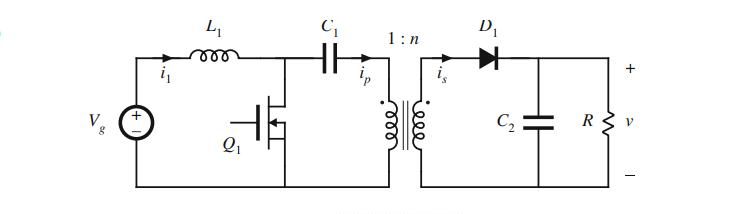
\includegraphics[width=\textwidth]{Figures/isolated_sepic.png}
    \caption{Isolated SEPIC Converter}
    \label{fig:iso_sepic}
\end{figure} \\
Some design considerations regarding isolated SEPIC converter can be stated as
\begin{itemize}
    \item The transformer acts similarly to the Flyback transformer, which sends power during off cycle.
    \item $C_1$ must be very large (ideally infinite).
    \item Assuming the previous requirement is met, $V_{C_1}$ $\approx$ $V_g$ and almost constant.
    \item Assuming $V_{C_1}$ = $V_g$, $I_{L_1}$ and $I_{L_m}$ have exactly the same voltage waveforms  during both the switch on and off cycles. If the magnetic design is done such that $L_1$ $\approx$ $L_m$, their current waveforms will almost be identical too. Therefore, measuring and controlling the current (if desired) from the input will be enough to control transformer current as well.
    \item $I_{Q_1}$ is approximately twice the input current during the on cycle, assuming $L_1$ $\approx$ $L_m$.
    \item Assuming ideal components, MOSFET blocking voltage can be found as $V_{Q_1}$ = $V_g$ + $V_o/n$. Overshoots during the switching instants must be considered as well.
\end{itemize}
The voltage transfer ratio for an isolated SEPIC converter can be stated as
\begin{equation*}
    \frac{V_o}{V_s} = \frac{N_2}{N_1}\frac{D}{1-D}
\end{equation*}
After evaluating positives and negatives we have decided to go for an isolated SEPIC converter design for the project.